%*************************************************************************
%	PLANTILLA PARA LA EDICIÓN DE PROYECTOS FIN DE CARRERA
%	Departamento de Teoría de la Señal y Comunicaciones
%	Universidad de Alcalá
%*************************************************************************

%******************
%Tipo de documento
%******************
%Descomentar la opción que corresponda:
%Versión durante la revisión (incluye números de línea)
\documentclass[12pt,twoside]{book}
\usepackage{lineno}
\linenumbers
%Versión final para imprimir a doble cara
%\documentclass[12pt,twoside]{book}
%Versión final para imprimir a una sola cara
%\documentclass[12pt,oneside]{book}

%********************
%Paquetes a utilizar
%********************

\usepackage[square,numbers]{natbib}
\usepackage[T1]{fontenc}
\usepackage[spanish]{babel}
\usepackage{verbatim}
\usepackage{amssymb}
\usepackage{amsmath}
\usepackage{fancyhdr}
\usepackage{graphicx}
\usepackage{multicol}
\usepackage{makeidx}
%\usepackage[bf,SL,BF]{subfigure}
\usepackage{subcaption}
\usepackage{caption}
\usepackage[utf8]{inputenc}
\usepackage{color}
\usepackage{multirow}
\usepackage{float}
\usepackage[printonlyused]{acronym}


\usepackage[pagebackref=true,breaklinks=true,letterpaper=true,colorlinks,bookmarks=false]{hyperref}
%No incluir paquetes depués de este.

%*************
%Definiciones
%*************
\deactivatetilden 
\addto\captionsspanish{\def\tablename{Tabla}\def\listtablename{Lista
de tablas}\def\listfigurename{Lista de figuras}}
%Cambios en los márgenes
\renewcommand{\baselinestretch}{1.1}

\setlength{\oddsidemargin}{0.4cm}
\setlength{\evensidemargin}{-0.4cm} \setlength{\headsep}{0.75cm}
\setlength{\textheight}{23cm} \setlength{\textwidth}{16cm}
\setlength{\topmargin}{-0.25cm}\flushbottom



%***************
%Título del TFC
%***************
\title{Sistema de adaptación inteligente de la velocidad para vehículos basado en IA y visión por computador}

%****************
%Autor
%****************
\author{Sergio Sastre Arrojo}

%Prepara el índice
\makeindex



%***********************
%Comienzo del documento
%***********************
\begin{document}
\setcounter{tocdepth}{4} \setcounter{secnumdepth}{3}

\frontmatter

%Incluimos fichero previo.tex -> genera la hoja de calificación y la portada
\begin{titlepage}
%**********************************************************
%GENERA LA HOJA OFICIAL DE CALIFICACIÓN PARA PROYECTOS FIN DE CARRERA
%SEGÚN EL FORMATO DE LA UNIVERSIDAD DE ALCALÁ Y DEL DEPAR-
%TAMENTO DE TEORÍA DE LA SEÑAL Y COMUNICACIONES.
%**********************************************************

\begin{center}
\LARGE \textsc{Universidad de Alcalá}\\
\vspace{0.5cm}

%Nombre de la escuela-> seleccione el que corresponda.
\textbf{Escuela Politécnica Superior}\\
%\textbf{Escuela Técnica Superior de Ingeniería Informática}\\

%Titulación -> escriba su titulación
Grado en Ingeniería Telemática
\end{center}

\vspace{0.5cm}

\begin{center}
%Para compilar con latex

\includegraphics[width=4cm]{Figuras/LogoUAH.eps}\\
%Para compilar con pdflatex
%
\includegraphics[width=4cm]{Figuras/LogoUAH.png}\\
\end{center}


\begin{center}
\vspace{1cm}

\LARGE Proyecto Fin de Carrera\\
\textbf{\Huge \textsc{{Sistema de adaptación de la velocidad para vehículos basado en IA y visión por computador}}}\\
\vspace{0.5cm}
\large Autor: Sergio Sastre Arrojo\\
Director: Roberto Javier López Sastre\\
\vspace{0.5cm}
\end{center}

\begin{flushleft}
\textbf{TRIBUNAL:}\\
\vspace{1.5cm}
\textit{Presidente: Manuel Utrilla Manso}\\
\vspace{1.5cm}
\textit{Vocal 1º: Pedro Gil Jiménez}\\
\vspace{1.5cm}
\textit{Vocal 2º: Roberto Javier López Sastre}\\
\vspace{1.5cm}
\textbf{CALIFICACIÓN:}............................................................ FECHA:.................... \\
%IMPORTANTE!
%La copia en PDF para la biblioteca, y uno de los tomos no lleva espacio para la PUBLICACIÓN!
\end{flushleft}
%Final de la hoja de calificación.

%Introduce hoja en blanco
\newpage
\thispagestyle{empty}
\hspace*{0.5cm}
\newpage


\end{titlepage}

%Prepara el título del proyecto.
\maketitle

%Introduce hoja en blanco
\newpage
\thispagestyle{empty}
\hspace*{0.5cm}
\newpage

%Incluye las dedicatorias (fichero dedicatorias.tex)
\begin{flushright}
\textit{Dedicado a mi familia, por haberme apoyado durante este largo camino.
A mis amigos, por haberme ayudado cuando más lo necesitaba.
A mis compañeros, con los que he compartido grandes momentos durante estos años de formación.
A mi tutor, por haber depositado su confianza en mí para este proyecto.
Y, en especial, a mis abuelos, por enseñarme a seguir adelante a pesar de las dificultades.}
\end{flushright}
%Introduce hoja en blanco
\newpage
\thispagestyle{empty}
\hspace*{0.5cm}
\newpage


%Incluye los agradecimientos (fichero agradecimientos.tex)
\chapter{Agradecimientos}
Gracias a todos los profesores y compañeros con los que me he cruzado y conocido durante una de las etapas más duras de mi vida, de los cuales he aprendido diferentes valores y me han enseñado cosas que, de otra forma, no hubiera aprendido. A mi familia, por criarme y educarme en la honestidad, la perseverancia, la resiliencia, y la satisfacción de un trabajo bien hecho. A mis amigos, por enseñarme el verdadero valor de la amistad al mostrarme su apoyo incondicional en situaciones tanto adversas como favorables.
%Siempre hay alguien a quien agradecerle algo, y más cuando has hecho un Proyecto Fin de Carrera (PFC).

%Introduce hoja en blanco
\newpage
\thispagestyle{empty}
\hspace*{0.5cm}
\newpage

%Inlcuimos el índice que latex genera automáticamente.
\tableofcontents
%La lista de figuras incluidas en el proyecto.
\listoffigures
%La lista de tablas.
\listoftables


%Incluye el resumen del Proyecto fin de carrera (fichero resumen.tex)
\chapter{Resumen}
%\textcolor{red}{Resumen de 100 palabras MÁXIMO}\\

En el siguiente trabajo vamos a tratar de solucionar un problema que lleva existiendo desde la invención del automóvil de una forma que no se había visto antes. Con la creación de las normas que regulan el tráfico en las carreteras y la fabricación masiva de vehículos, es un hecho que la probabilidad de que ocurra un accidente es muy alta. Para solucionarlo se inventaron los sistemas \ac{ISA} \cite{reduccion} que ayudaron a reducir este número... Sin embargo, no son perfectos y tienen fallos.

Es por ello que aquí sugerimos nuestra solución con un nuevo y mejorado sistema: \[ISA^{2}\]
%TODO: Sergio, esto es un abstract o resumen, y debes resumir el trabajo. Lo que has puesto no es un resumen. Hay que explicar, muy brevemente, en qué consiste la solucion propuesta. Mira por ejemplo el Abstract/Resumen del artículo de congreso. Cuando lo tengas en castellano lo traduces al inglés y lo subes.

\vspace{0.5cm}

\textbf{Palabras clave}: visión por computador, inteligencia artificial, sistema de adaptación de la velocidad inteligente, vehículos inteligentes.
%\textbf{Palabras clave}: cinco palabras como máximo, separadas por comas.

%Introduce hoja en blanco
\newpage
\thispagestyle{empty}
\hspace*{0.5cm}
\newpage

\chapter{Abstract}
%\textcolor{red}{Resumen de 100 palabras MÁXIMO - Es OBLIGATORIO}\\



\vspace{0.5cm}

\textbf{Keywords}: computer vision, artificial intelligence, intelligent speed adaptation, intelligent vehicles.
%\textbf{Keywords}: cinco palabras como máximo, separadas por comas.
%Introduce hoja en blanco
\newpage
\thispagestyle{empty}
\hspace*{0.5cm}
\newpage


%Incluye el resumen Extendido del Proyecto fin de carrera (fichero resumen-extendido.tex)
\chapter{Resumen Extendido}
%Debe incluir un resumen del trabajo de un máximo de 5 páginas. Resaltar aspectos fundamentales del desarrollo, los resultados más relevantes y las conclusiones.

El principal objetivo que persigue este trabajo fin de grado es mostrar y mejorar el sistema $ISA^{2}$ que presentaremos más adelante. Este sistema tiene como fin ser una alternativa para los ya existentes sistemas \ac{ISA}, puesto que éstos tienen una serie de fallos que solucionar y están enfocados de manera diferente.

La principal diferencia de $ISA^{2}$ con estos sistemas reside en cuál es la base de éste. Los sistemas \ac{ISA} están basados en tecnología \ac{GPS} y sensores de proximidad para con otros vehículos, mientras que la propuesta $ISA^{2}$ simplemente utiliza imágenes tomadas desde una cámara, y modelos de inteligencia artificial, para ser capaz de indicar al conductor la velocidad a la que debe circular.

En resumen, el sistema $ISA^{2}$ comienza capturando una imagen de la escena de tráfico que observa un vehículo. Sobre esta imagen se realiza un proceso de \ac{SS}. La \ac{SS} se puede explicar como el procedimiento de inteligencia artificial que es capaz de predecir qué clases (etiquetas) hay en una imagen, para cada uno de sus píxeles. Pero, ¿qué es una clase? O mejor dicho, ¿cómo definimos una clase en este contexto? Una clase (o etiqueta) es la forma de categorizar una parte de la imagen para diferenciarla de otras. Dicho de otra forma, sirve para que un programa sepa de qué partes se compone una imagen. Se hace dándole un mismo valor a un conjunto de píxeles en concreto, para distinguirlos de los demás \cite{deeplab}.

\begin{figure}[H]
  \centering
  \includegraphics[width=8cm]{Figuras/Ejemplo_Imagen_Segmentada.eps}
  \caption{Imagen Segmentada}
    \label{fig:ImgSegm}
\end{figure}

En la Figura \ref{ImgSegm} puede verse un ejemplo de segmentación semántica como la que utiliza nuestro modelo $ISA^{2}$. Una vez se ha completado la segmentación semántica, se utiliza esta información para entrenar un conjunto de regresores que son capaces de aprender a estimar la velocidad a la que debe ir el vehículo.

En este proyecto hacemos uso del modelo de deep learning \textbf{Swiftnet} \cite{swiftnet} para conseguir la segmentación semántica. \textbf{Swiftnet} es la base sobre la que desarrollamos este proyecto y donde más hemos trabajado para conseguir los resultados de las velocidades estimadas.

Swiftnet es un modelo de \textbf{tiempo real} que recibe imágenes de la vía cada cierto tiempo. Una vez las va recibiendo, va procesándolas una a una y predice una máscara de segmentación semántica en cada una de ellas, con una gran precisión.

Para trabajar con Swiftnet, previamente tenemos que construir el ``escenario'' sobre el que se va a ejecutar, y para ello nos servimos de un entorno \textbf{Conda} \cite{conda}. No entraremos, aún, en detalle sobre la explicación de Conda, pero sí diremos que nos sirve para crear un entorno virtual con todos los requerimientos necesarios para trabajar con Swiftnet.

Una vez lo creamos, siguiendo los pasos que más adelante explicaremos, conseguiremos replicar los resultado de Swiftnet tal y como se detallan en el artículo original \cite{swiftnet}, empleando el software que proporcionan los propios autores \cite{github_swiftnet}.

%Pero todavía no hemos terminado con Swiftnet, puesto que lo hemos ejecutado con una base de datos compuesta por imágenes que no se corresponde a la que se usó en la primera versión de $ISA^{2}$.

Una vez tenemos el modelo de segmentación semántica Swiftnet funcionando, pasamos a aplicarlo al problema propuesto. Por ello, debemos descargar la base de datos de $ISA^{2}$ y aplicar los cambios pertinentes en Swiftnet para que funcione en la misma, generando una máscara de segmentación semántica para cada imagen en $ISA^{2}$. Una vez lo conseguimos, debemos generar una serie de histogramas \cite{histograma} que recojan las clases de cada imagen procesada por Swiftnet, replicando el modelo propuesto en el artículo \cite{isa2}. Para generarlos nos serviremos de unos códigos en \textbf{MatLab} \cite{matlab}.

Con los histogramas creados, ya podemos ejecutar los sistemas de regresión para la parte final del proyecto: la estimación de la velocidad, y la comparación de la misma con la velocidad real de las imágenes (anotada en la base de datos $ISA^{2}$) . Todo esto lo hacemos replicando el modelo experimental descrito en \cite{isa2}, donde se proponen varias soluciones de inteligencia artificial para resolver el problema de la adaptación de la velocidad inteligente en base a imágenes.

\begin{figure}[H]
  \centering
  \includegraphics[width=8cm]{Figuras/Figura_Esquema_ISA2_Version_2.eps}
  \caption{Esquema $ISA^{2}$}
  \label{fig:isa2}
\end{figure}

En la figura \ref{isa2} puede verse la solución global propuesta, desde la segmentación semántica con Swiftnet hasta la aplicación del modelo de regresión para la estimación de la velocidad.

%TODO_DONE: Añade figura/diagrama explicativa de todo el sistema.

Según nuestros experimentos, los sistemas con mejores resultados, a pesar de que sean solo en entornos urbanos, son los que emplean \textit{Boosting Trees} \cite{boosting-trees} y \textit{\ac{SVR}} \cite{SVR}, como se puede ver en la tabla \ref{tab:Resul_Resumen}:

\begin{table}[H]
\centering
\resizebox{12cm}{!}{
\begin{tabular}{|l|l|l|l|l|}\cline{1-5}
& \multicolumn{2}{|l|}{\textbf{MAE Swiftnet}} & \multicolumn{2}{|l|}{\textbf{MAE DeepLab}} \\ \cline{1-5}
\textbf{Regresión} & \textbf{Highway (\%)} & \textbf{Urban (\%)} & \textbf{Highway (\%)} & \textbf{Urban (\%)}\\ \cline{1-5}
\textbf{\textit{Boosting Trees}} & 13.43 & \textbf{9.83} & 11.35 & \textbf{10.14} \\ \cline{1-5}
\textbf{\textit{SVR}} & 11.13 & \textbf{8.74} & 9.69 & \textbf{9.55} \\ \cline{1-5}
\end{tabular}
}
\caption{Resultados de Boosting Trees y \ac{SVR}}
\label{tab:Resul_Resumen}
\end{table}

En la tabla anterior hemos puesto los valores del \ac{MAE} más bajos, es decir, más precisos; calculados por dichos sistemas de regresión.

Nótese cómo particularmente en \textit{\ac{SVR}}, el margen de mejora con respecto a \textbf{DeepLab} (modelo usado en la primera versión) es de casi un 1\% (0.8\%). Por otro lado, \textit{Boosting Trees} es algo ``peor'' que \textit{\ac{SVR}} debido al poco margen de mejora que tiene (0.3\%).

Sin embargo, es importante destacarlo ya que el resto de sistemas son considerablemente menos precisos:

\begin{table}[H]
\centering
\resizebox{12cm}{!}{
\begin{tabular}{|l|l|l|l|l|}\cline{1-5}
& \multicolumn{2}{|l|}{\textbf{MAE Swiftnet}} & \multicolumn{2}{|l|}{\textbf{MAE DeepLab}} \\ \cline{1-5}
\textbf{Regresión} & \textbf{Highway (\%)} & \textbf{Urban (\%)} & \textbf{Highway (\%)} & \textbf{Urban (\%)}\\ \cline{1-5}
\textbf{\textit{Lasso}} & 12.90 & 9.23 & 11.29 & 8.43 \\ \cline{1-5}
\textbf{\textit{Linear}} & 12.22 & 8.95 & 10.32 & 8.38 \\ \cline{1-5}
\end{tabular}
}
\caption{Resultados de Lasso y Linear}
\label{tab:Resul_Resumen_LL}
\end{table}

Como se puede observar en la tabla \ref{tab:Resul_Resumen_LL}, tanto el sistema \textit{Lasso} como \textit{Linear} tienen buenos resultados en entornos urbanos, pero en comparación con DeepLab, no tienen un margen de mejora como tal. Dicho de otra forma, tienen un margen de mejora negativo.

A continuación podemos ver los resultados de las tablas gráficamente en las siguientes figuras:

\begin{figure}[H]
  \centering
  \begin{subfigure}[b]{0.45\linewidth}
    \includegraphics[width=\linewidth]{Figuras/Lineal_Highway(Nivel_1).eps}
    \caption{Highway con Linear}
  \end{subfigure}
    \begin{subfigure}[b]{0.425\linewidth}
    \includegraphics[width=\linewidth]{Figuras/Lasso_Highway(Nivel_1).eps}
    \caption{Highway con Lasso}
  \end{subfigure}
    \begin{subfigure}[b]{0.45\linewidth}
    \includegraphics[width=\linewidth]{Figuras/Boosting_Urban(Nivel_1).eps}
    \caption{Urban con Boosting Trees}
  \end{subfigure}
      \begin{subfigure}[b]{0.45\linewidth}
    \includegraphics[width=\linewidth]{Figuras/SVR_Urban(Nivel_1).eps}
    \caption{Urban con SVR}
  \end{subfigure}
  \caption{Resultados gráficos}
\end{figure}

Analizando estos resultados, vemos cómo los datos en los sistemas \textit{Lineal} y \textit{Lasso} son prácticamente idénticos. Esto es porque ambos están actuando en imágenes de autovías, donde Swiftnet no lo hace tan bien como DeepLab. En las tablas anteriores se puede ver cómo ésto no sólo es así usando estos dos sistemas, lo es para todos ellos, porque Swiftnet en ese tipo de entornos es peor que DeepLab.

No obstante, sí es mejor en un entorno en el que hay que tener una gran precisión para determinar qué elementos forman parte del mismo en cada momento: los núcleos urbanos.

Como se puede apreciar en las gráficas, la similitud entre la parte real (línea \textbf{azul}) y la estimada (línea \textbf{roja}) para los sistemas \textit{Boosting Trees} y \textit{\ac{SVR}} es más que evidente. Ambos sistemas son muy acertados para grandes urbes y cabría destacar más aún el propio \ac{SVR}, basándonos en los datos recogidos en la tabla \ref{tab:Resul_Resumen} y los mostrados en su gráfica. Que un sistema registre un \ac{MAE} tan bajo (8.74\%) para una zona urbana, denota que Swiftnet es el modelo adecuado para este proyecto.

%TODO_DONE: Añade más detalles sobre los números. Hay que resumir en un par de párrafos el capítulo de resultados.
%TODO_DONE: Añade resultados en gráficas.
%TODO_DONE: Añade resultados cualitativos.

De todos estos experimentos cabe destacar un hecho muy importante: Swiftnet, a diferencia de \textbf{DeepLab} (el modelo de \ac{SS} de la primera versión publicado en \cite{isa2}), es un modelo \textbf{Real-Time}, es decir, el coste de su implementación es mucho menor y, por si no fuera suficiente, trabaja mejor en entornos urbanos.

Por todo ello, y para concluir, podemos decir que: aunque DeepLab trabaje mejor en autovías y autopistas, Swiftnet lo compensa haciéndolo mejor en entornos urbanos, lo cual es más complejo por la dificultad que tiene el poder clasificar con gran precisión tan diferentes y variadas etiquetas en un mismo escenario. Además, cabe recordar que Swiftnet es un modelo Real-Time, de modo que la velocidad con la que procesa los datos es superior que la del modelo DeepLab (además del coste de implementación del propio modelo que ya hemos explicado con anterioridad). Finalmente, hemos visto la precisión en la estimación de la velocidad de Swiftnet observando las tablas y gráficas anteriores usando como métrica el \ac{MAE}, y se ha comprobado de forma cuantitativa cuánto mejor es éste con respecto a DeepLab para escenarios más complejos.
%TODO_DONE: Añade más conclusiones, sobre velocidad, precisión en la estimación, etc.


%Incluimos lista de abreviaturas
\chapter{Glosario}

%Lista con los acrónimos
\begin{acronym}[PFC]
\item \acro{PFC}{Proyecto Fin de Carrera}
\end{acronym}

\begin{acronym}[ISA]
\item \acro{ISA}{Intelligent Speed Adaptation}
\end{acronym}

\begin{acronym}[SS]
%\item \acro{SS}{Proceso por el cual los píxeles de una imagen son dotados de distintos valores para poder diferenciarlos en etiquetas unos de otros y así reconocer los elementos que componen dicha imagen. Por ejemplo: Una fotografía de una persona, un coche y un perro. A priori, todos los píxeles de la imagen no están categorizados y no se sabe qué partes de la imagen corresponden a la persona, al coche, y al perro. Gracias a la segmentación semántica los píxeles de la imagen adquieren los valores de las etiquetas referentes a "persona", "coche" y "perro"; y son fácilmente diferenciables.}
\item \acro{SS}{Segmentación Semántica}
\end{acronym}

\begin{acronym}[mIoU]
\item \acro{mIoU}{Mean Intersection Over Union}
\end{acronym}

\begin{acronym}[IoU]
\item \acro{IoU}{Intersection Over Union}
\end{acronym}

\begin{acronym}[CNN]
%\item \acro{CNN}{Tecnología que posibilita la predicción de etiquetas de una imagen para la segmentación semántica}
\item \acro{CNN}{Convolutional Neural Network}
\end{acronym}

\begin{acronym}[SI]
\item \acro{SI}{Spatial Information}
\end{acronym}

\begin{acronym}[SPP]
\item \acro{SPP}{Spatial Pyramid Pooling}
\end{acronym}

\begin{acronym}[ABI]
\item \acro{ABI}{Application Binary Interface}
\end{acronym}

\begin{acronym}[GPU]
\item \acro{GPU}{Graphical Processing Units}
\end{acronym}

\begin{acronym}[CPU]
\item \acro{CPU}{Central Processing Units}
\end{acronym}

\begin{acronym}[IDE]
\item \acro{IDE}{Integrated Development Environment}
\end{acronym}

\begin{acronym}[MAE]
\item \acro{MAE}{Mean Absolute Error}
\end{acronym}

\begin{acronym}[SVR]
\item \acro{SVR}{Support Vector Regression}
\end{acronym}

\begin{acronym}[SVM]
\item \acro{SVM}{Support Vector Machine}
\end{acronym}
%Para poner más acrónimos
%\acrodef{CNN}{Convolutional Neural Network}
%\acrodef{SS}{Segmentación Semántica}







\mainmatter

%Incluimos los capítulos del proyecto. Cada capitulo se encuentra en un fichero tex,
%que insertamos en el documento por medio del comando \include{capitulo-cualquiera}

%Incluye Introducción (fichero introduccion.tex)
% Formato para un capítulo cualquiera

%Título del capítulo
\chapter{Introducción} 


Durante todo el siglo XX, en España, han ocurrido más de 7.000.000 de accidentes de tráfico \cite{sigloXX}, de los que en aproximadamente en 250.000 ha habido víctimas mortales \cite{vidas}. Un siglo después, gracias a la evolución de la tecnología, se crean los sistemas \ac{ISA}, que permiten establecer una velocidad aproximada para ayudar al conductor en cualquier situación de la vía.
%TODO: No me convence el párafo, pasas de los accidentes a los ISA dando un gran salto. Los sistemsa ISA no han aparecido un siglo después, por cierto, llevan tiempo. Modifica el párrafo para hilar ambas cosas. ¿Cuántos accidentes se deben a excesos de velocidad? ¿Hay cifras? Regular la velocidad es importante, existen lo sistemas ISA. Habla de soluciones comerciales (hay muchos modelos de coches que los llevan, basados en sistemas de detección de señales de tráfico, GPS y meta información, sensores de proximidad, etc).


Con la creación de estos sistemas se estima que el número de accidentes se reduciría considerablemente, y más importante aún, el número de víctimas \cite{reduccion}.


Sin embargo, estos sistemas, a pesar de tener buenas prestaciones, poseen fallos que pueden derivar en posibles accidentes. Esto es debido a que la mayoría de sistemas \ac{ISA} están basados en \ac{GPS} y en adaptación por proximidad de vehículos y objetos, y como se puede prever, no son unas bases lo suficientemente sólidas como para proporcionar un mayor grado de seguridad en el conductor; ya que tienen fallos sujetos a la situación del tráfico y de la zona en la que se encuentran en un instante, todo ello sin hablar de las condiciones climáticas que haya en ese momento.


Es por ello que aquí presentamos nuestro sistema capaz de resolver (en gran medida) estos problemas: \[ISA^{2}\]


\section{¿Qué es $ISA^{2}$? ¿Cómo funciona?}


La principal novedad de $ISA^{2}$ frente a los otros sistemas \ac{ISA} reside en la capacidad para analizar el tráfico, en un determinado momento, y predecir, en consecuencia, la velocidad apropiada para ese instante.


Para ello usamos una cámara en la parte frontal del vehículo que va tomando fotos con una cierta cadencia. Gracias a un sistema de \ac{SS}, conseguimos saber qué es cada cosa en cada foto, es decir; qué píxeles son los correspondientes a un vehículo, peatón, semáforo, acera, etc,... Más tarde lo explicaremos con más detalle.


En función de qué detecte, es capaz de estimar con gran precisión la velocidad a la que se requiere ir para ese instante.


He aquí un ejemplo de una imagen real \ref{fig:ImgOrig} y de la misma imagen procesada por el sistema de \ac{SS} \ref{fig:ImgSegm}:

\begin{figure}[h]
  \centering
  \includegraphics[width=12cm]{Figuras/Imagen_Original.eps}
  \caption{Imagen Original}
  \label{fig:ImgOrig}
\end{figure}

\begin{figure}[h]
  \centering
  \includegraphics[width=12cm]{Figuras/Ejemplo_Imagen_Segmentada.eps}
  \caption{Imagen Segmentada}
    \label{fig:ImgSegm}
\end{figure}


\section{Objetivo principal}


El objetivo principal de este proyecto es la optimización del sistema $ISA^{2}$ y para ello lo que hemos hecho ha sido un largo proceso de análisis de sistemas de \ac{SS}, acompañado de la dificultad que éstos conllevan para poder ejecutarlos correctamente. Tras ello, hemos recogido los datos generados por dicho sistema, los hemos evaluado para obtener las velocidades correspondientes, y hemos comparado éstas con las de la primera versión de $ISA^{2}$, obteniendo resultados muy prometedores.


En la primera versión se utilizó un framework llamado \textbf{DeepLab} \cite{deeplab} para realizar el proceso de segmentación semántica con unos resultados muy buenos. Para este proyecto, a través de una exhaustiva búsqueda de modelos y tras muchas pruebas, hemos utilizado uno conocido como \textbf{Swiftnet} \cite{swiftnet}, el cual conlleva una mejora realmente interesante.

Afortunadamente, Swiftnet es un modelo de código abierto en GitHub de modo que cualquiera puede utilizarlo a su disposición \cite{github_swiftnet}. Todo lo que hay que hacer es clonar el repositorio en el que se encuentra utilizando el siguiente comando en la terminal del sistema \cite{clonar}:

\begin{center}
\textit{git clone URL\_del\_repositorio}
\end{center}

Cuando clonemos el repositorio, se recomienda hacerlo desde el escritorio (carpeta \textbf{Desktop}) para ejecutar Swiftnet según este trabajo.

En el siguiente capítulo, explicaremos en detalle el proceso que realiza $ISA^{2}$ parte por parte, y los pasos que hemos seguido para conseguir que todo funcione correctamente.

\section{Campos de aplicación}


Este proyecto será aplicable a cualquier campo relacionado con el automovilismo, para ayudar a mejorar la seguridad vial actual y para facilitar la lectura de la vía durante la conducción. A modo de resumen, podríamos plasmar las ideas recogidas de todo lo anterior en los siguientes puntos:
\begin{enumerate}	
	\item Implementación de soluciones de adaptación de velocidad inteligente.
	\item Implementación de sistema de detección de situaciones peligrosas en función de la velocidad.
	\item Desarrollo de nuevas ayudas a la conducción más inteligentes.
\end{enumerate}

\section{Medios disponibles}

Dispondremos de las siguientes herramientas:

\begin{enumerate}
	\item Estación de trabajo con \textbf{GPU (NVIDIA 1080 TI)} para la realización de experimentos con sistema operativo \textbf{Ubuntu}.
	\item Acceso a la librería de \textbf{Deep Learning} llamada \textbf{PyTorch} \cite{pytorch}
	\item Acceso a la base de datos $ISA^2$ utilizada en la primera versión \cite{isa2} a través del siguiente enlace: \url{http://agamenon.tsc.uah.es/Personales/rlopez/data/isa2/index.html}.
\end{enumerate}
%\section{¿Cómo escribir tu PFC en \LaTeX{} ?}

%Escribir un \ac{PFC} es una tarea de gran importancia. La herramienta de edición \LaTeX{} te va a permitir editar tu \ac{PFC} de una forma elegante, útil y segura. Simplemente dedicando unos minutos a comprender cómo están organizados los ficheros que acabas de descargar, y realizando algunas pruebas con ellos, podrás comenzar a escribir el tuyo.

%\subsection{La mejor manera para aprender a programar es programando}

%\LaTeX{} es un lenguaje de programación como tantos otros a los que estás acostumbrado. Puedes encontrar mucha información y manuales en Internet, siendo el mejor sitio \cite{LatexWiki}. También te recomiendo las referencias siguientes: \cite{Latex1} y \cite{Latex2}.

%Este documento PDF que estás leyendo ha sido generado mediante \LaTeX{} utilizando los ficheros:
%\begin{enumerate}
%\item \textit{tfc.tex} : es el fichero principal, desde él se hacen las llamadas a los demás ficheros, que pueden ser editados de forma independiente. Si abres este fichero con cualquier editor de textos verás que contiene muchas sentencias que ahora desconoces. Puedes observar que el fichero tiene una zona de cabecera donde se incluyen todos los paquetes a utilizar. Luego se define el título del documento y su autor, para, al final, ir añadiendo los capítulos y secciones de tu \ac{PFC}.
%\item \textit{previo.tex}: genera la hoja de calificación oficial para un \ac{PFC} de la Universidad de Alcalá.
%\item \textit{dedicatoria.tex}: para que escribas tus dedicatorias.
%\item \textit{agradecimientos.tex}: para que escribas los agradecimientos, que seguro son muchos.
%\item \textit{resumen.tex}: aquí debes escribir un resumen de tu trabajo.
%\item \textit{introduccion.tex}: este es un capítulo modelo, en el que encontrarás los comandos utilizados para generar lo que estás ahora mismo leyendo.
%\item \textit{apendice-a.tex}: un modelo de apéndice, muy utilizado en un \ac{PFC} cuando queremos incluir en el documento final código fuente, manuales de usuario, \ldots
%\item \textit{bibliografia-pfc.bib} : este es un fichero \textit{.bib} (no lleva la extensión .tex como los anteriores). Es un fichero de bibliografía \textbf{BibTex}. La bibliografía es una parte fundamental de un \ac{PFC}, y es por ello que debemos poner especial cuidado a la hora de editarla, ya que va a permitir que futuros lectores de tu \ac{PFC}, que seguro serán muchos, puedan acudir a las referencias cuando no entiendan algo, o cuando pretendan retomar tu trabajo y continuar con él para mejorarlo. Sobre BibTex también existen muchos manuales, pero encontrarás información útil en \cite{bibtex1}. Para manejar tu bibliografía te recomiendo el programa JabRef\footnote{En Ubuntu está disponible, o si prefieres, puedes descargar la última versión de la página oficial \url{http://jabref.sourceforge.net/}}.
%\end{enumerate}

%Para probar que todo esto funciona sólo tienes que compilar el fichero \textit{tfc.tex}, ¿pero cómo?. %Evidentemente necesitas un compilador. Veamos que opciones existen:

%\begin{enumerate}
%\item \textbf{\underline{Plataforma Linux (Unix)}}: simplemente necesitas tener instalado el compilador \textit{latex}, que suele estar incluido en un paquete con el mismo nombre. Existe un entorno de trabajo bastante agradable y útil, que es \textit{Kile}, sobre el que podrás editar tus documentos de forma cómoda, gráfica y sencilla. También puedes utilizar la herramienta \textit{Lyx}, que te permite saber cómo va quedando tu documento a medida que escribes, sin necesidad de primero editar el código y luego compilar, es decir, es un software de filosofía WYSIWYM (What You See Is What You Mean).
%\item \textbf{\underline{Otras plataformas}}: para trabajar con \LaTeX{} sobre otros sistemas operativos dispones de gran cantidad de software. Simplemente voy a indicarte algunas herramientas que son de libre distribución:
%\begin{itemize}
%\item Compilador: el único que conozco es \textit{MikTex}, lo puedes descargar de su web oficial.
%\item Editor: puedes utilizar TeXnicCenter o WinShell, ambos de libre distribución.
%\end{itemize}
%\end{enumerate}

%Una sugerencia: \textbf{\textit{¿no crees que es un buen momento para trabajar desde Linux?}}. Si no tienes este sistema operativo en tu ordenador, prueba a instalar la distribución \textit{Ubuntu} (http://www.ubuntu.com), es realmente sencillo funcionar con ella, y además puedes descargarla desde la web o incluso pedir un cd de forma totalmente gratuita.


%Ahora que conoces algunas herramientas, debes probar a compilar el fichero \textit{tfc.tex} hasta que obtengas como resultado este pdf.

%\subsection{Algunos detalles más}

%Con \LaTeX{} puedes editar tus propias tablas (Tabla \ref{tabla:primera}), e incluso añadir gráficos a tus documentos (Figura \ref{grafico:primero}). A la hora de añadir un gráfico la mejor opción es trabajar con formatos de imagen \textit{.eps}, vectorial preferiblemente, aunque puedes incrustar imágenes en formato bmp, jpg y otros muchos.

%\begin{table}
%\begin{center}
%\begin{tabular}{|c|c|c|}\hline
%\textbf{Medida} & \textbf{Error} & \textbf{Porcentaje} \% \\ \hline
%12 & 23.6 & 22 \\ \hline
%-1 & 13 & 4 \\ \hline
%6 & 3 & 4 \\ \hline
%\end{tabular}
%\caption[El título corto de la tabla.]{El título de la tabla.}
%\label{tabla:primera}
%\end{center}
%\end{table}

%\begin{figure}
%\begin{center}
%Para compilar con latex
%
\includegraphics[width=4cm]{Figuras/LogoUAH.eps}\\
%Para compilar con pdflatex
%
\includegraphics[width=4cm]{Figuras/LogoUAH.png}\\
%\end{center}
%\caption[El título corto de la gráfica.]{El título de la gráfica.}
%\label{grafico:primero}
%\end{figure}


%\LaTeX{} también te permite editar ecuaciones de forma muy sencilla y realmente elegante, observa.
%\begin{equation}
%I = \! \int_{-\infty}^\infty f(x)\,dx \label{eq:fine}.
%\end{equation}

%\begin{equation}
%\label{eq:mdiv}
%m(T) =
%\begin{cases}
%0 & \text{$T > T_c$} \\
%\bigl(1 - [\sinh 2 \beta J]^{-4} \bigr)^{\! 1/8} & \text{$T < T_c$}
%\end{cases}
%\end{equation}

%\begin{align}
%\textbf{T} &=
%\begin{pmatrix}
%T_{++} \hfill & T_{+-} \\
%T_{-+} & T_{--} \hfill 
%\end{pmatrix} , \nonumber \\
%& =
%\begin{pmatrix}
%e^{\beta (J + B)} \hfill & e^{-\beta J} \hfill \\
%e^{-\beta J} \hfill & e^{\beta (J - B)} \hfill
%\end{pmatrix}.
%\end{align}

%\section{Recomendaciones importantes}
%Antes de enviarme un copia de tu trabajo para revisar, asegúrate de que has realizado las siguientes tareas:
%\begin{enumerate}
 %\item Pasar un corrector ortográfico. Kile trae uno incorporado. No seguiré revisando ningún documento que contenga más de 3 faltas de ortografía.
 %\item Leer lo que hemos escrito y revisarlo hasta que tenga coherencia. No seguiré revisando ningún documeto que contenga más de 3 frases que no se entiendan.
 %\item Todas la figuras que se incluyen deben citarse en el texto. Lo mismo ocurre con las tablas. Debes aprender a manejar los comandos \verb+\label+ y \verb+\ref+.
 %\item La Bibliografía es FUNDAMENTAL. Cita bien y cita mucho.  Debes aprender a manejar el comando \verb+\cite+ y a tener una base de datos con todas tus lecturas en formato BibTex.
 %\item En la redacción del proyecto procura mantener un estilo serio. Se trata de un documento oficial.
%\end{enumerate}


%\section{Para terminar}
%En el fichero \textit{introduccion.tex} encontrarás todo el código que se ha utilizado para generar este capítulo, échale un vistazo y trata de entender todo aquello que está escrito en él. Si consigues generar este documento pdf de nuevo, es que estás preparado para editar tu propio \ac{PFC} incluyendo los nuevos capítulos que necesites.

%\begin{center}
%\begin{large}\textbf{Adelante y buena suerte.}\end{large}
%\end{center}



%Incluye un capítulo cualquiera (capitulo-cualquiera.tex)
\chapter{$ISA^{2}$}

Hemos hablado anteriormente de qué son los sistemas \ac{ISA} a grandes rasgos y la principal novedad de $ISA^{2}$ frente a éstos, pero conviene entrar en detalle para explicar la metodología que hemos seguido y los problemas que nos hemos encontrado y solventado.

\section{Estructura de $ISA^{2}$}

Para poder explicar la metodología, antes debemos de preguntarnos cómo funciona todo el sistema de $ISA^{2}$, centrándonos en cada parte que lo compone para que resulte más fácil su comprensión. He aquí unas figuras ilustrativas que nos servirán como punto de referencia durante todo el capítulo:


\begin{figure}[h]
  \centering
  \includegraphics[width=8cm]{Figuras/Figura_Esquema_ISA2_Version_1_SegSem.eps}
  \caption{Esquema $ISA^{2}$ Antiguo}
  \label{fig:Isa_v1}
\end{figure}


Como se puede ver al pie de la figura \ref{fig:Isa_v1}, este fue el esquema utilizado para la primera versión de $ISA^{2}$ \cite{isa2} y funcionaba de la siguiente manera:


\begin{itemize}
\item En primera instancia el sistema recogía un set de imágenes que se correspondía con situaciones de tráfico tanto en autovía (o autopista) como en núcleos urbanos. Cuando el sistema tenía que procesar una imagen, ésta venía en diferentes escalas puesto que el modelo de ``DeepLab'' de \ac{SS} trabajaba así. Este modelo tenía como base una \ac{CNN}, es decir, una Red Neuronal Convolucional \cite{cnn}.
 
\item Este tipo de tecnología es la que posibilitó entonces, y ahora, la \ac{SS} de las imágenes.

\subsection{Segmentación Semántica}

Pero, ¿qué es la \ac{SS}? ¿Y por qué es tan útil en este proyecto?


En el capítulo anterior hablamos de una forma resumida en qué consiste la \ac{SS} y su uso en el proyecto, pero es tan solo la punta del iceberg.


La \ac{SS} es un proceso por el cual los píxeles de una imagen son dotados de distintos valores para poder diferenciarlos en etiquetas unos de otros y así reconocer los elementos que componen dicha imagen. 


Por ejemplo: Una fotografía de una persona, un coche y un perro. A priori, todos los píxeles de la imagen no están categorizados y no se sabe qué partes de la imagen corresponden a la persona, al coche, y al perro. Gracias a la segmentación semántica los píxeles de la imagen adquieren los valores de las etiquetas referentes a ``persona'', a ``coche'' y a ``perro''; y son fácilmente diferenciables.

Cuando hablamos de ``diferenciables'' nos referimos a los programas y soluciones que trabajan con este tipo de tecnologías. Más adelante usaremos unos códigos en MatLab que trabajan con estas etiquetas, pero es conveniente saber el porqué de esa ``diferenciabilidad'' a la que se hace alusión.

\item Tras este proceso, mediante unos códigos de Matlab se recogían los datos de los píxeles ya segmentados y se organizaban en histogramas. Basándonos en los histogramas generados, usábamos una estrategia llamada \ac{SPP} \cite{spp} para crear un descriptor de imagen.

\item Por último, el descriptor generado en el paso anterior se pasaba a diferentes sistemas de regresión. Para cada uno de ellos se añadía \ac{SI} \cite{spp} usando \ac{SPP} de hasta 3 niveles para poder compararlos entre sí y saber cuál era mejor. Para ello cogíamos los mejores resultados de cada uno de todos los niveles usados en los mismos.

\end{itemize}


Fue de esta manera como se pudo ejecutar con eficacia este sistema \cite{isa2}. Sin embargo, con el paso de los años surgieron nuevos modelos de \ac{SS} más eficaces y precisos, y fruto de ello es el sistema que hemos utilizado en esta nueva versión: Swiftnet \cite{swiftnet}.


\begin{figure}[H]
  \centering
  \includegraphics[width=8cm]{Figuras/Figura_Esquema_ISA2_Version_2.eps}
  \caption{Esquema $ISA^{2}$ Actual}
    \label{fig:Isa_v2}
\end{figure}


Como se puede comprobar, el esquema de la figura \ref{fig:Isa_v2} sigue el mismo camino que el de la primera versión, salvo por unas modificaciones al principio que pasamos a explicar a continuación:

\begin{enumerate}

\item Las imágenes de entrada al modelo de \ac{SS} no llegan en diferentes escalas como se podría intuir. La razón de por qué es así es ``Swiftnet'': El modelo admite tanto imágenes en diferente escala como imágenes en una única.


Sin embargo, para este proyecto hemos optado por la recomendación de los autores \cite{github_swiftnet} y hemos decidido hacerlo con una única escala. De esta manera hemos obtenido los resultados esperados con la dataset de Cityscapes \cite{cityscapes} que ellos mismos utilizaron \cite{swiftnet}.

\item La segunda, y última, modificación es la más obvia: la sustitución del modelo de ``DeepLab'' \cite{deeplab} por el modelo de ``Swiftnet'' \cite{swiftnet}.

A diferencia del primero, ``Swiftnet'' es un modelo que opera en tiempo real (``Real-Time'') de tal modo que cuando procesa una imagen lo hace en el momento, mientras que ``DeepLab'' tiene que esperar a que se recoja un set de imágenes para luego ir procesándolas.

\end{enumerate}


En el siguiente capítulo hablaremos acerca de la implementación de ``Swiftnet'' y de cómo es mejor para los campos de aplicación, especificados anteriormente, con respecto a ``DeepLab''.

\include{Implementación}

\chapter{Resultados}

En la siguiente tabla pasamos a mostrar los resultados tanto de la versión anterior de $ISA^{2}$ como de la actual. Como ya dijimos anteriormente, el \ac{MAE} será la métrica que usaremos para esta tarea, pues indica cuánta precisión ha habido en la \ac{SS} realizada por el modelo Swiftnet \cite{swiftnet} con respecto al modelo DeepLab \cite{deeplab}.

Recordemos que, a raíz de la \ac{SS} realizada por uno de los modelos, generamos los histogramas que, posteriormente, se usaron en los sistemas de regresión para estimar la velocidad apropiada; de modo que el \ac{MAE} es una métrica muy acertada para saber qué versión del proyecto es mejor.

\begin{table}[H]
\centering
\resizebox{16cm}{!}{
\begin{tabular}{|l|l|l|l|l|l|}\cline{1-6}
& & \multicolumn{2}{|l|}{\textbf{MAE Swiftnet}} & \multicolumn{2}{|l|}{\textbf{MAE DeepLab}} \\ \cline{1-6}
\textbf{Regresión} & \textbf{Nivel de \ac{SPP}} & \textbf{Highway (\%)} & \textbf{Urban (\%)} & \textbf{Highway (\%)} & \textbf{Urban (\%)}\\ \cline{1-6}
\multirow{3}{*}{\textbf{\textit{Linear}}} & 1 & 12.22 & 8.95 & 10.32 & 8.38 \\ \cline{2-6}
& 2 & 13.94 & 9.45 & 11.18 & 8.81 \\ \cline{2-6}
& 3 & 13.39 & \textbf{\textit{11.79}} & 15.5 & \textbf{\textit{10.83}}\\ \cline{1-6}
\multirow{3}{*}{\textbf{\textit{Lasso}}} & 1 & 12.90 & 9.23 & 11.29 & 8.43 \\ \cline{2-6}
 & 2 & 13.80 & 9.40 & 11.7 & 8.62 \\ \cline{2-6}
 & 3 & 13.47 & 10.16 & 10.8 & 9.25\\ \cline{1-6}
\multirow{3}{*}{\textbf{\textit{Boosting Trees}}} & 1 & 13.43 & \textbf{9.83} & 11.35 & \textbf{10.14} \\ \cline{2-6}
 & 2 & 14.97 & \textbf{10.52} & 12.23 & \textbf{10.72}\\ \cline{2-6}
 & 3 & 14.75 & \textbf{10.08} & 10.37 & \textbf{10.12}\\ \cline{1-6}
\multirow{3}{*}{\textbf{\textit{SVR}}} & 1 & 11.13 & \textbf{8.74} & 9.69 & \textbf{9.55} \\ \cline{2-6}
 & 2 & 12.24 & \textbf{8.98} & 9.98 & \textbf{9.09}\\ \cline{2-6}
 & 3 & 12.09 & \textbf{9.60} & 9.78 & \textbf{9.62}\\ \cline{1-6}
\end{tabular}
}
\caption{Tabla de resultados}
\end{table}

Como se puede apreciar, para cada modelo de \ac{SS} se han segmentado imágenes correspondientes a autovías (o autopistas) y a entornos urbanos.

Los valores de Swiftnet que aparecen \textbf{resaltados de esta forma} indican que son mejores que los valores de DeepLab (\textbf{también resaltados}) para esa fila.

Por otro lado, hemos puesto dos valores con \textit{\textbf{este aspecto}} para indicar que, durante la predicción de la velocidad en el sistema de regresión lineal, hemos modificado un parámetro para obtener unos resultados más apropiados; ya que, de otra forma, se obtendrían valores muy lejanos a la realidad.

Como se puede observar, tanto los sistemas \textit{Boosting Trees} como \textit{\ac{SVR}} son mejores con la nueva versión para entornos urbanos, mientras que para las autovías es mejor utilizar el modelo DeepLab. Esto quiere decir que Swiftnet trabaja mejor con entornos en los que se requiere más nivel de detalle y DeepLab, por el contrario, lo realiza mejor en entornos más abiertos.

Cabe destacar que Swiftnet \cite{swiftnet} es un modelo \textbf{Real-Time}, de modo que su implementación es menos que costosa que DeepLab, el cual, por el contrario, necesita de un tiempo de procesamiento para realizar su función.

A continuación mostramos algunas figuras con las que podemos ver, de forma gráfica, los resultados de los sistemas de regresión con la \ac{SS} realizada por Swiftnet:

\begin{figure}[H]
  \centering
  \begin{subfigure}[b]{0.45\linewidth}
    \includegraphics[width=\linewidth]{Figuras/Lineal_Highway(Nivel_1).eps}
    \caption{Highway con Lineal en nivel 1 de \ac{SPP}}
  \end{subfigure}
    \begin{subfigure}[b]{0.425\linewidth}
    \includegraphics[width=\linewidth]{Figuras/Lasso_Urban(Nivel_1).eps}
    \caption{Urban con Lasso en nivel 1 de \ac{SPP}}
  \end{subfigure}
    \begin{subfigure}[b]{0.45\linewidth}
    \includegraphics[width=\linewidth]{Figuras/Boosting_Urban(Nivel_1).eps}
    \caption{Urban con Boosting en nivel 1 de \ac{SPP}}
  \end{subfigure}
      \begin{subfigure}[b]{0.45\linewidth}
    \includegraphics[width=\linewidth]{Figuras/SVR_Urban(Nivel_1).eps}
    \caption{Urban con SVR en nivel 1 de \ac{SPP}}
  \end{subfigure}
  \caption{Resultados gráficos}
\end{figure}

En las figuras, los puntos azules representan la velocidad \textbf{real} a la que debe ir el vehículo en cada imagen, mientras que los puntos rojos representan la velocidad \textbf{estimada} por los sistemas de regresión en cada imagen.

Como se puede observar, hemos escogido, en su mayoría, aquellas figuras en las que los sistemas de regresión han dado mejores resultados, es decir, en entornos urbanos \textbf{(Urban)}. Sin embargo, para contrastar cómo trabaja Swiftnet en autovías hemos decidido poner una figura con esos datos (\textbf{Highway}).

Hemos visto cómo se realiza todo el proceso de este trabajo y hemos comparado los resultados actuales con los anteriores. A continuación, finalizaremos con las conclusiones de éste.

\chapter{Conclusiones}

En este trabajo hemos contribuido a la evolución del sistema $ISA^{2}$ como respuesta a los sistemas \ac{ISA} ya existentes \cite{isa2}. Hemos podido comprobar cómo al implementar un modelo \textbf{Real-Time} con una mayor precisión para la \ac{SS} (Swiftnet \cite{swiftnet}), el propio sistema mejora en aspectos muy importantes, entre los que destacan:

\begin{itemize}
\item Mayor precisión en entornos urbanos para la estimación de la velocidad.
\item Menor tiempo de procesado, lo que posibilita la integración del sistema en un vehículo inteligente.
\end{itemize}

%De modo que, usando este modelo, con las variaciones que ello conlleva, podemos asegurar que este sistema es mejor que su predecesor.

En la siguiente tabla \ref{tab:Resul_SVR} comprobamos que esto es así mostrando el mejor resultado del modelo en núcleos urbanos en comparación con DeepLab utilizando el mismo sistema de regresión (\ac{SVR}): 

\begin{table}[H]
\centering
\resizebox{12cm}{!}{
\begin{tabular}{|l|l|l|l|l|}\cline{1-5}
& \multicolumn{2}{|l|}{\textbf{MAE Swiftnet}} & \multicolumn{2}{|l|}{\textbf{MAE DeepLab}} \\ \cline{1-5}
\textbf{Regresión} & \textbf{Highway (\%)} & \textbf{Urban (\%)} & \textbf{Highway (\%)} & \textbf{Urban (\%)}\\ \cline{1-5}
\textbf{\textit{SVR}} & 11.13 & \textbf{8.74} & 9.69 & \textbf{9.55} \\ \cline{1-5}
\end{tabular}
}
\caption{Resultados de \ac{SVR}}
\label{tab:Resul_SVR}
\end{table}

Podemos comprobar que, efectivamente, Swiftnet (\textbf{8.74\%}) es mejor que DeepLab (\textbf{9.55}) en términos de \ac{MAE} para estos escenarios, aportando una mayor rapidez de procesado de imágenes (9 \ac{FPS} para analizar la base de datos de $ISA^{2}$) y un menor coste de implementación del mismo en un vehículo inteligente (por ser un modelo Real-Time). 

%TODO_DONE: Modifica esta frase, no me convence, y pon una comparativa explícita con el anterior modelo en términos de MAE, de modo que el lector termine el documento sabiendo cuanto mejor es la solución propuesta que el anterior. Añade también información sobre la velocidad del sistema en frames por segundo.

Por todo ello, concluimos con la idea de que esta nueva versión de $ISA^{2}$ sirva como punto de referencia para futuras mejoras del mismo. Como futuras líneas de trabajo proponemos las siguientes:

\begin{itemize}
\item La sustitución del modelo Swiftnet por otro con mayor precisión (por ejemplo \cite{hierarchical-multiscale}).
\item La posibilidad de añadir nuevos sistemas de regresión al esquema (como por ejemplo \cite{ridge}).
\item Un nuevo esquema con una estructura diferente para $ISA^{2}$, por ejemplo uno basado en una arquitectura con \ac{CNN} que realice la regresión por sí misma, como se hizo en la primera versión del sistema \cite{isa2}, usando nuevas arquitecturas \cite{cnn-ss}.
\end{itemize}
%TODO_DONE: Añade, bosqueja, algunas líneas de mejora que se deriven de tu trabajo. Pueden/deben ser muy técnicas.

Al principio de este trabajo, contamos cómo con los sistemas \ac{ISA} se habían reducido cuantiosamente el número de accidentes de tráfico en España y Europa. Con este sistema, y con los que se deriven de éste, esperemos que, en un futuro no muy lejano, esa cifra deje de existir.



%Prepara la sección de apéncices, si es que se necesita.
%\appendix
%% Formato para un capítulo cualquiera

%Título del capítulo
\chapter{CÓDIGO FUENTE.} 
%Sección primera
\section{Primera sección del apéndice.}
Texto de la primera sección.
\subsection{Segunda sección del apéndice.}
Texto de la segunda sección.
\subsubsection{Tercera sección del apéndice.}
Texto de la tercera sección.

%\include{fichero-apendice-b}


\backmatter

\nocite{*}



%*****************************
%Sección para la bibliografía
%*****************************

%Posibles estilos de bibliografia
\bibliographystyle{plain}
%\bibliographystyle{abbrvnat}
%\bibliographystyle{klunamed}
%\bibliographystyle{unsrt}

\addcontentsline{toc}{chapter}{{}Bibliografía}

%Toma los datos del fichero bibliografia-pfc.bib
\bibliography{bibliografia-pfc}

%\printindex

\end{document}

%Final de la plantilla.